\documentclass[a4paper,12pt]{report}

%Русский язык
\usepackage[T2A]{fontenc}
\usepackage[utf8]{inputenc}
\usepackage[english,russian]{babel}
\usepackage{cmap}

%Работа с кодом
\usepackage{listings}
\usepackage{color}

\definecolor{green}{rgb}{0,0.6,0}
\definecolor{gray}{rgb}{0.5,0.5,0.5}
\definecolor{red}{rgb}{0.6,0,0}

\lstset{
        language=Python, 
        basicstyle=\small\ttfamily, 
        numberstyle=\tiny,           
        columns=flexible,
        stepnumber=1,                   
        numbersep=5pt,        
        showspaces=false,
        showstringspaces=false,
        showtabs=false,
        tabsize=2,                
        captionpos=b,              
        breaklines=true,           
        breakatwhitespace=false,
        keywordstyle=\color{green},
        commentstyle=\color{gray},
        stringstyle=\color{red},      
}

%Математика
\usepackage{amsmath,amsfonts,amssymb,amsthm,mathtools} 

%Изображения
\usepackage{float}
\usepackage{graphicx}
\graphicspath{ {./img/} }

%Поля страницы
\usepackage{geometry} 
\geometry{left=2.3cm} 
\geometry{right=1.8cm} 
\geometry{top=2cm} 
\geometry{bottom=2.5cm} 

%Отступы
\usepackage{indentfirst}
\setlength{\parskip}{0cm}

\begin{document} 

\begin{titlepage}
\newpage
	\begin{center}
		\large Санкт-Петербургский политехнический университет Петра Великого\\
		Институт компьютерных наук и технологий\\
		Высшая школа интеллектуальных систем и суперкомпьютерных технологий\\
	\end{center}
\vspace{7cm}

\begin{center}
		\large \textbf{Отчёт по лабораторной работе №4} \\
		\textbf{Дисциплина:} Телекоммуникационные технологии\\
		\textbf{Тема:} Шум
\end{center}
\vspace{4cm}
	
\begin{flushright}
		\large Работу выполнил:\\ Ляшенко В.В.\\
		Группа: 3530901/80201\\
		Преподаватель:\\ Богач Н.В.
\end{flushright}

\vspace{\fill}
\begin{center}
	\large Санкт-Петербург\\ 2021
	\end{center}
\end{titlepage}

\tableofcontents
\listoffigures
\lstlistoflistings

\chapter{Упражнение 4.1}
    Скачаем с сайта \texttt{https://freesound.org} несколько примеров шума: шум огня в камине и стрекот сверчков. Затем вычислим их спектры.
    
\section{Камин}
    Начнем с шума огня.
\begin{lstlisting}[caption=Выделение сегмента]
       from thinkdsp import read_wave

       wave = read_wave('sounds/132534__inchadney__fireplace.wav')
       segment = wave.segment(start=0, duration=1.0)
       segment.make_audio()
\end{lstlisting}
    
    Получим спектр этого сегмента (Рис.1.1).
\begin{lstlisting}[caption=Получение спектра]
       spectrum = segment.make_spectrum()
       spectrum.plot_power()
       decorate(xlabel='Frequency (Hz)')
\end{lstlisting}
\begin{figure}[H]
        \centering
        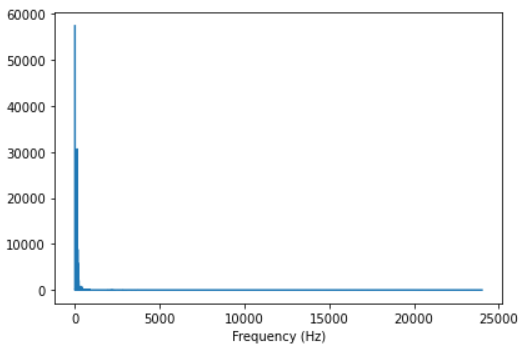
\includegraphics[width=0.8\textwidth]{fig1-1.PNG}
        \caption{Спектр звука}
        \label{fig:fig1-1}
\end{figure} 
    
    Амплитуда падает с частотой, поэтому это либо красный шум, либо розовый. Мы можем проверить это, посмотрев на спектр мощности в логарифмической шкале.
\begin{lstlisting}[caption=Получение спектра в логарифмической шкале]
       spectrum.plot_power()
       loglog = dict(xscale='log', yscale='log')
       decorate(xlabel='Frequency (Hz)', **loglog)
\end{lstlisting}
\begin{figure}[H]
        \centering
        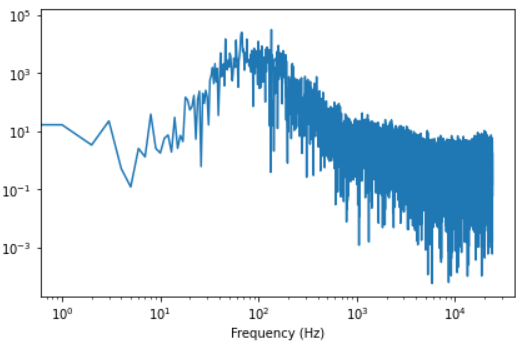
\includegraphics[width=0.8\textwidth]{fig1-2.PNG}
        \caption{Спектр мощности}
        \label{fig:fig1-2}
\end{figure}
    
    На рис.1.2 мы можем видеть, что амплитуда сначала увеличивается, а потом уменьшается, что является обычным для естественных источников шума.
    
    Теперь построим спектрограмму.
\begin{lstlisting}[caption=Получение спектрограммы]
       segment.make_spectrogram(256).plot(high=2000)
       decorate(xlabel='Time(s)', ylabel='Frequency (Hz)')
\end{lstlisting}
\begin{figure}[H]
        \centering
        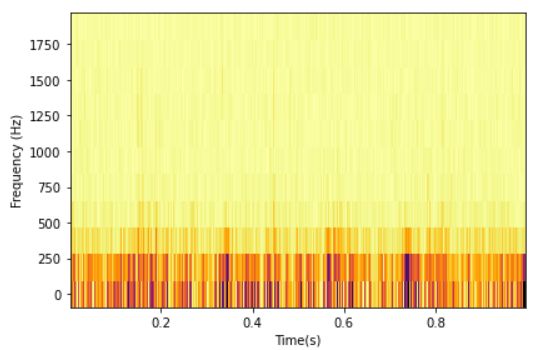
\includegraphics[width=0.8\textwidth]{fig1-3.PNG}
        \caption{Спектрограмма звука}
        \label{fig:fig1-3}
\end{figure}

    Из рис.1.3 можно сделать вывод, что это белый шум.
\section{Сверчки}
    Теперь проанализируем стрекотание сверчков.
\begin{lstlisting}[caption=Выделение сегмента]
       from thinkdsp import read_wave

       wave = read_wave('sounds/22604__martypinso__dmp010037-crickets-texas.wav')
       segment = wave.segment(start=0, duration=1.0)
       segment.make_audio()
\end{lstlisting}

    Получим спектр этого сегмента (Рис.1.4).
\begin{lstlisting}[caption=Получение спектра]
       spectrum = segment.make_spectrum()
       spectrum.plot_power()
       decorate(xlabel='Frequency (Hz)')
\end{lstlisting}
\begin{figure}[H]
        \centering
        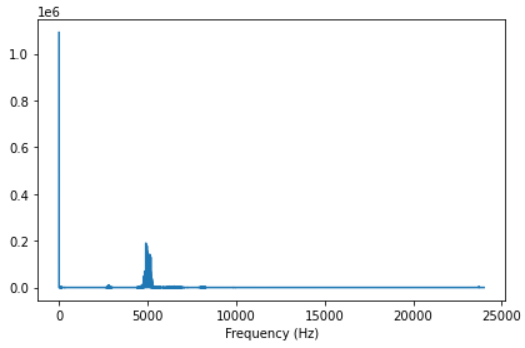
\includegraphics[width=0.8\textwidth]{fig1-4.PNG}
        \caption{Спектр звука}
        \label{fig:fig1-4}
\end{figure} 
    
    Посмотрим на спектр мощности в логарифмической шкале.
\begin{lstlisting}[caption=Получение спектра в логарифмической шкале]
       spectrum.plot_power()
       loglog = dict(xscale='log', yscale='log')
       decorate(xlabel='Frequency (Hz)', **loglog)
\end{lstlisting}
\begin{figure}[H]
        \centering
        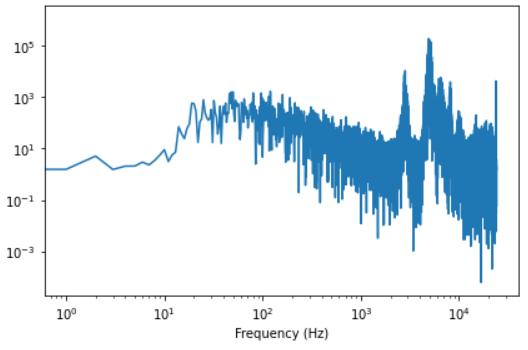
\includegraphics[width=0.8\textwidth]{fig1-5.PNG}
        \caption{Спектр мощности}
        \label{fig:fig1-5}
\end{figure}
    
    Из рис.1.5 мы можем предположить, что это либо розовый шум, либо белый.
    
    Теперь построим спектрограмму.
\begin{lstlisting}[caption=Получение спектрограммы]
       segment.make_spectrogram(256).plot(high=2000)
       decorate(xlabel='Time(s)', ylabel='Frequency (Hz)')
\end{lstlisting}
\begin{figure}[H]
        \centering
        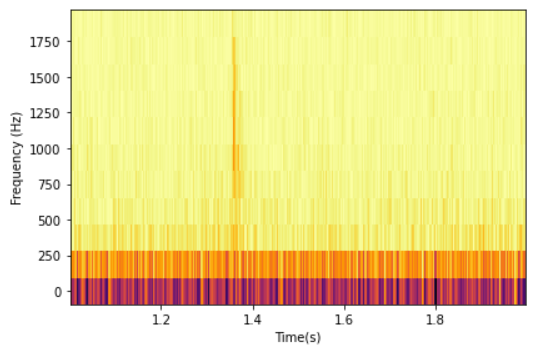
\includegraphics[width=0.8\textwidth]{fig1-6.PNG}
        \caption{Спектрограмма звука}
        \label{fig:fig1-6}
\end{figure}

    Из рис.1.6 можно сделать вывод, что это белый шум.
    
\chapter{Упражнение 4.2}
\section{Метод Бартлетта}
    Реализуем метод Бартлетта.
\begin{lstlisting}[caption=Метод Бартлетта]
from thinkdsp import Spectrum

def bartlett_method(wave, seg_length=512, win_flag=True):
    spectro = wave.make_spectrogram(seg_length, win_flag)
    spectrums = spectro.spec_map.values()
    
    psds = [spectrum.power for spectrum in spectrums]
    
    hs = np.sqrt(sum(psds) / len(psds))
    fs = next(iter(spectrums)).fs
    
    spectrum = Spectrum(hs, fs, wave.framerate)
    return spectrum
\end{lstlisting}

\section{Использование метода}    
    Затем используем его для оценки спектра мощности шумового сигнала. Для этого создадим два сегмента одного сигнала. Пусть это будет шум огня в камине.
\begin{lstlisting}[caption=Использование метода]
       wave = read_wave('sounds/22604__martypinso__dmp010037-crickets-texas.wav')
       segment1 = wave.segment(start=1.0, duration=1.0)
       segment2 = wave.segment(start=2.5, duration=1.0)

       bart1 = bartlett_method(segment1)
       bart2 = bartlett_method(segment2)

       bart1.plot_power()
       bart2.plot_power()

       decorate(xlabel='Frequency (Hz)', ylabel='Power', **loglog)
\end{lstlisting} 
\begin{figure}[H]
        \centering
        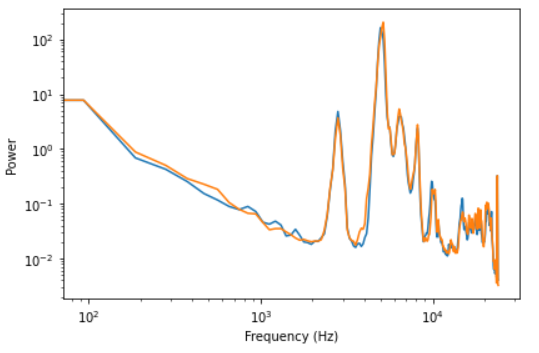
\includegraphics[width=0.8\textwidth]{fig2-1.PNG}
        \caption{Соотношение мощности и частоты}
        \label{fig:fig2-1}
\end{figure}

    На рис.2.1 мы можем видеть, что мощность и частота взаимосвязаны. Их взаимосвязь не линейна, а имеет необычныую форму. Но для разных сегментов она одинакова.

\chapter{Упражнение 4.3}
    Скачаем с сайта \texttt{http://www.coindesk.com} исторические данные о ежедневной цене BitCoin. Откроем этот файл и вычислим спектр цен BitCoin как функцию времени.
    Вначале нам необходимо загрузить данные (Рис.3.1). 
\begin{lstlisting}[caption=Получение данных о BitCoin]
       import pandas as pd

       df = pd.read_csv('files/BTC_USD_2020-04-12_2021-04-11-CoinDesk.csv')
       df
\end{lstlisting}
\begin{figure}[H]
        \centering
        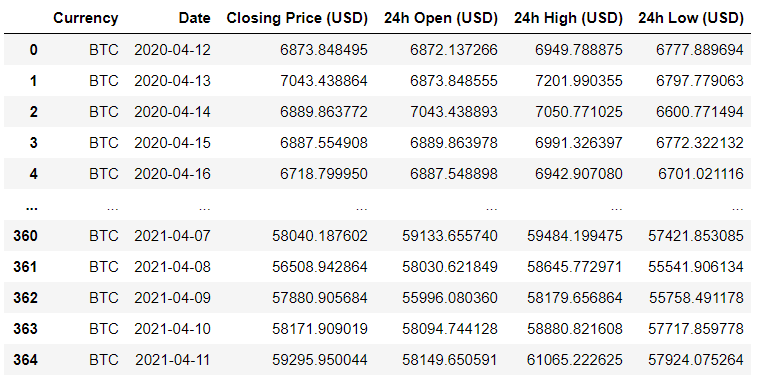
\includegraphics[width=0.8\textwidth]{fig3-1.PNG}
        \caption{Данные о BitCoin}
        \label{fig:fig3-1}
\end{figure}
    
    Представим данные в виде графика (Рис.3.2).                                
\begin{lstlisting}[caption=Представление данных в виде графика]
       from thinkdsp import Wave
       
       ys = df['Closing Price (USD)']
       ts = df.index
       wave = Wave(ys, ts, framerate=1)
       wave.plot()
       decorate(xlabel='Time (days)')
\end{lstlisting}
\begin{figure}[H]
        \centering
        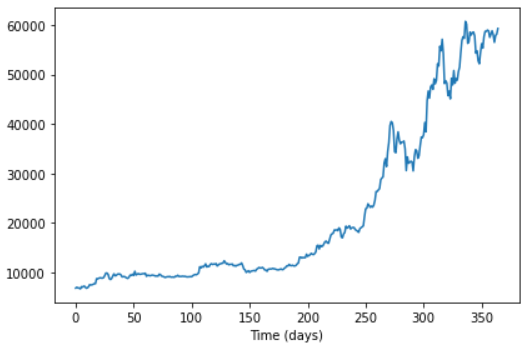
\includegraphics[width=0.8\textwidth]{fig3-2.PNG}
        \caption{График данных о BitCoin}
        \label{fig:fig3-2}
\end{figure}

    Получим спектр BitCoin.
\begin{lstlisting}[caption=Вычисление спектра BitCoin]
       spectrum = wave.make_spectrum()
       spectrum.plot_power()
       decorate(xlabel='Frequency (1/days)', **loglog)
\end{lstlisting}
\begin{figure}[H]
        \centering
        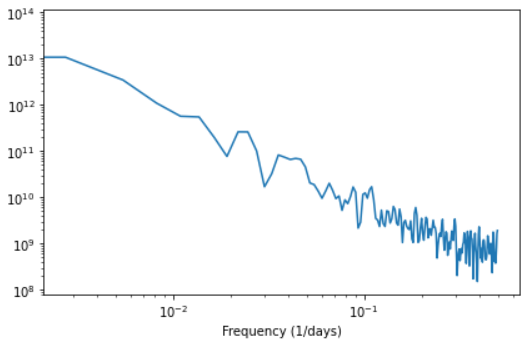
\includegraphics[width=0.8\textwidth]{fig3-3.PNG}
        \caption{Спектр BitCoin}
        \label{fig:fig3-3}
\end{figure}

    Из рис.3.3 мы можем предположить, что это либо красный, либо розовый шум. Чтобы определить более точно, вычислим угол наклона графика.
\begin{lstlisting}[caption=Вычисление угла наклона]
       spectrum.estimate_slope()[0]
\end{lstlisting}

    Красный шум должен иметь наклон -2. Наклон этого графика имеет значение примерно -1,7, поэтому трудно сказать, следует ли считать этот красным шумом или розовым.
    
\chapter{Упражнение 4.4}
\section{Класс UncorrelatedPoissonNoise}
    Напишем класс \texttt{UncorrelatedPoissonNoise}, наследующий \texttt{thinkdsp.\_Noise} и предоставляющий \texttt{evaluate}.
\begin{lstlisting}[caption=Класс UncorrelatedPoissonNoise]
from thinkdsp import Noise

class UncorrelatedPoissonNoise(Noise):

    def evaluate(self, ts):
        ys = np.random.poisson(self.amp, len(ts))
        return ys
\end{lstlisting}

\section{Получение звука}
    Сгенерируем пару секунд UP и послушаем. Сначала зададим маленькое значение \texttt{amp}.
\begin{lstlisting}[caption=Получение звука при малых значениях amp]
       signal1 = UncorrelatedPoissonNoise(amp=0.0005)
       wave1 = signal1.make_wave(duration=1, framerate=10000)
       wave1.plot()
       wave1.make_audio()
\end{lstlisting}
    
    При малых значениях \texttt{amp} звук как у счётчика Гейгера. График сигнала представлен на рис.4.1.
\begin{figure}[H]
        \centering
        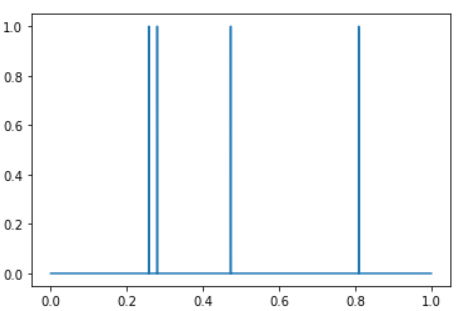
\includegraphics[width=0.8\textwidth]{fig4-1.PNG}
        \caption{График при малом amp}
        \label{fig:fig4-1}
\end{figure}
    
    Вычислим ожидаемое и полученное количество частиц, чтобы убедиться в корректности работы.
\begin{lstlisting}[caption=Число частиц при малых значениях amp]
       expected = 0.0005 * 10000 * 1
       actual = sum(wave1.ys)
       print(expected, actual)
\end{lstlisting} 

    Ожидаемое число = 5, полученное = 4. Значения близки к друг другу, значит, всё верно.
    
    Теперь зададим большое значение \texttt{amp}.       
\begin{lstlisting}[caption=Получение звука при больших значениях amp]
       signal2 = UncorrelatedPoissonNoise(amp=1)
       wave2 = signal2.make_wave(duration=1, framerate=10000)
       wave2.plot()
       wave2.make_audio()
\end{lstlisting}  

      При больших значениях звук похож на белый шум. График сигнала представлен на рис.4.2.
\begin{figure}[H]
        \centering
        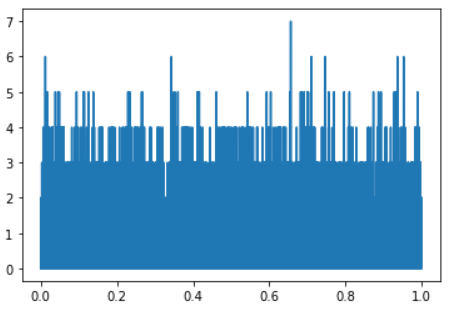
\includegraphics[width=0.8\textwidth]{fig4-2.PNG}
        \caption{График при большом amp}
        \label{fig:fig4-2}
\end{figure}
    
    Так же вычислим ожидаемое и полученное количество частиц, чтобы убедиться в корректности работы.
\begin{lstlisting}[caption=Число частиц при малых значениях amp]
       expected = 1 * 10000 * 1
       actual = sum(wave1.ys)
       print(expected, actual)
\end{lstlisting} 

    Ожидаемое число = 10000, полученное = 10046. При больших значениях всё тоже в порядке. 
\section{Спектр мощности}
    Вычислим и напечатаем спектры мощности обоих сигналов.
\begin{lstlisting}[caption=Вычисление спектров мощности]
       spectrum1 = wave1.make_spectrum()
       spectrum2 = wave2.make_spectrum()

       spectrum1.plot_power(alpha=0.5)
       spectrum2.plot_power(alpha=0.5)
       decorate(xlabel='Frequency (Hz)', ylabel='Power', **loglog)
\end{lstlisting}
\begin{figure}[H]
        \centering
        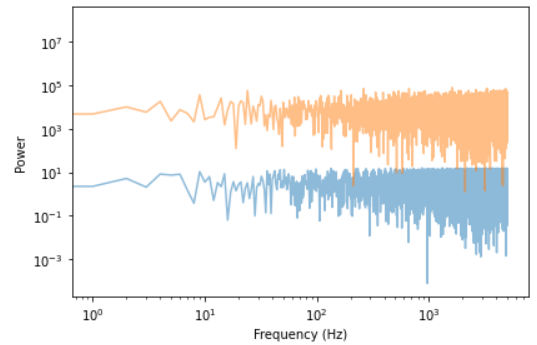
\includegraphics[width=0.8\textwidth]{fig4-3.PNG}
        \caption{Спектры мощности}
        \label{fig:fig4-3}
\end{figure} 

    Как мы можем видеть на рис.4.3, графики почти идентичны. К тому же, они не имеют наклона, так что их можно отнести к белому шуму.   
 
\chapter{Упражнение 4.5}
\section{Алгоритм Voss-McCartney}
    Реализуем алгоритм Voss-McCartney для генерации розового шума и вычислим спектр результата. 
\begin{lstlisting}[caption=Алгоритм Voss-McCartney]
       def voss(nrows, ncols=16):
       array = np.empty((nrows, ncols))
       array.fill(np.nan)
       array[0, :] = np.random.random(ncols)
       array[:, 0] = np.random.random(nrows)
    
       n = nrows
       cols = np.random.geometric(0.5, n)
       cols[cols >= ncols] = 0
       rows = np.random.randint(nrows, size=n)
       array[rows, cols] = np.random.random(n)

       data = pd.DataFrame(array)
       data.fillna(method='ffill', axis=0, inplace=True)
       total = data.sum(axis=1)

       return total.values
\end{lstlisting}

    Чтобы проверить работу метода сгененрируем 20000 значений и построим график (Рис.5.1).
\begin{lstlisting}[caption=Генерация розового шума]
       from thinkdsp import Wave
       wave = Wave(voss(20000))
       wave.unbias()
       wave.normalize()
       wave.plot()
       wave.make_audio()
\end{lstlisting}
\begin{figure}[H]
        \centering
        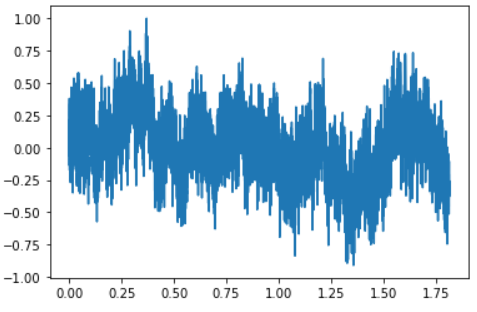
\includegraphics[width=0.8\textwidth]{fig5-1.PNG}
        \caption{Шум}
        \label{fig:fig5-1}
\end{figure} 

    Послушаем данный звук и убедимся, что он действительно похож на шум.
    
    Теперь построим спектр мощности.
\begin{lstlisting}[caption=Получение спектра мощности]
       spectrum = wave.make_spectrum()
       spectrum.hs[0] = 0
       spectrum.plot_power()
       decorate(xlabel='Frequency (Hz)', **loglog)
\end{lstlisting}
\begin{figure}[H]
        \centering
        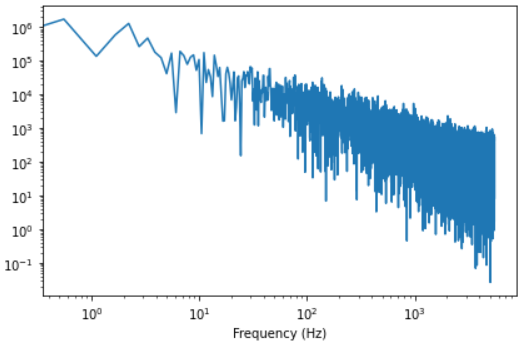
\includegraphics[width=0.8\textwidth]{fig5-2.PNG}
        \caption{Спектр мощности}
        \label{fig:fig5-2}
\end{figure} 

    Как мы можем видеть на рис.5.2, это действительно похоже на розовый шум. Чтобы в этом точно убедиться, расчитаем наклон с помощью \texttt{spectrum.estimate\_slope().slope}. Полученное значение можно округлить до -1. Значит, точно получен розовый шум.
\section{Соотношение между мощностью и частотой}
    Теперь необходимо убедиться, что соотношение между мощностью и частотой соответствующее. Для этого мы сгенерируем более длинную выборку и используем метод Бартлетта.
\begin{lstlisting}[caption=Создание выборки]
       seg_length = 64 * 2048
       wave = Wave(voss(seg_length * 100))
       len(wave)
\end{lstlisting}

    Полученное значение: 13107200.
    
    Применим метод Бартлетта.
\begin{lstlisting}[caption=Использование метода Бартлетта]
       spectrum = bartlett_method(wave, seg_length=seg_length, win_flag=False)
       spectrum.hs[0] = 0
       len(spectrum)
\end{lstlisting}  

    Полученное значение: 65537.
    
    Построим график соотношения мощности и частоты.
\begin{lstlisting}[caption=Построение соотношения мощности и частоты]
       spectrum.plot_power()
       decorate(xlabel='Frequency (Hz)', ylabel='Power', **loglog)
\end{lstlisting}
\begin{figure}[H]
        \centering
        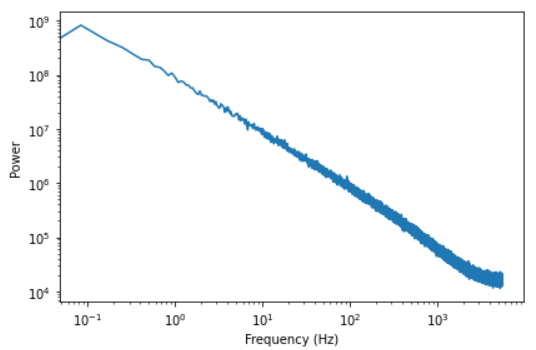
\includegraphics[width=0.8\textwidth]{fig5-3.PNG}
        \caption{Соотношение мощности и частоты}
        \label{fig:fig5-3}
\end{figure} 

    На рис.5.3 мы можем видеть, что взаимосвязь мощности и частоты похожа на прямую.
    
    Вычислим её наклон с помощью \texttt{spectrum.estimate\_slope().slope}. При округлении получается -1.

\chapter{Выводы}
    В результате выполнения данный работы мы познакомились с различными видами шумов и для работы с ними изучили метод Бартлетта и алгоритм Voss-McCartney.
    
    Метод Бартлетта используется для оценки спектров мощности, а алгоритм Voss-McCartney позволяет генерировать розовый шум.
\end{document}
\end{document}